\documentclass[a4paper]{article}

\usepackage{INTERSPEECH_v2}
\usepackage{animate}

\title{HMM Weather Modelling}
\name{Victor Jiao$^1$}
\address{
  $^1$University of Chicago, USA}
\email{victorjiao@cs.uchicago.edu}

\begin{document}

\maketitle
% 
\begin{abstract}

Modern weather forecasting is largely accomplished through the use of highly sophisticated and complex physics-based weather simulations run on data retrieved from a network of satellites and official weather stations. Although there has been research done in applying neural networks of various types (GANs, RNNs, CNNs) to predicting certain aspects of weather, particularly rainfall, there hasn't been much research into applying basic statistical models to more general weather data. 

In this paper, I visualize and examine daily weather data from the past 60 years at 4 airports in the US, fit HMMs of different hidden classes to the data with the Baum-Welch algorithm, and test the quality of the model by comparing its 1-day forecasting accuracy with naive forecasting and historical weather forecasting statistics. 

I chose to use HMMs as my main model because they are relatively transparent (as compared to many neural network implementations) and simple in operation, while the hidden states in an HMM offers an additional layer of depth to the model in parsing the data.

In additional to the main test with learning HMM parameters from the 20-odd-dimensional weather data, I also attempted to modulate the weather data in various ways to attempt to increase the resultant model's 1-day forecasting accuracy. These different transformations included training on data without strongly temporal dimensions, data where each point has the past week of data concatenated onto it, and data where each point represents the linear change in weather statistics from the previous day. Only one of these methods (the final 'delta' method) routinely beat the 'naive' method, where we assume tomorrow's weather is the same as today's.
\end{abstract}

\noindent\textbf{Index Terms}: weather prediction, clustering, hidden markov models




\section{Introduction and Motivation}


Modern meteorology and weather forecasting generally relies on running physical simulations using official national weather data. This relies heavily on the quality and quantity of the data used. In the United States, the national weather services that make official weather forecasts use data taken directly from satellites and official weather stations, so they are as accurate as possible. However, these models and techniques are severely limited by the amount of computational power they are given and the level of accuracy with which programmers can replicate atmospheric behavior. Small errors in the model or data can lead to huge systematic errors in certain situations and longer-distance forecasting.

However, weather follows more predictable patterns on smaller scales too --- it isn't necessary to look at the entire world's current weather status (plus a few days of weather history) to make a reasonable prediction for whether it'll rain later today or not. 

There are two main kinds of weather locality that we can exploit --- temporal and spatial. Weather has temporal locality because weather is continuous, and although day-to-day weather can still change drastically, we can generally expect weather between days to be similar in most characteristics most of the time. Weather also has spatial locality because of two reasons --- firstly, weather in two different locations are oftentimes similar depending on how similar their climates are, and secondly, storms and air masses generally move around instead of staying put. For example if it rained nearby yesterday, it is more likely that it'll rain today than if there was no nearby rain yesterday. 

This paper focuses mostly on analyzing different ways of attempting to access that spacial locality.

\begin{figure}[t]
  \centering
  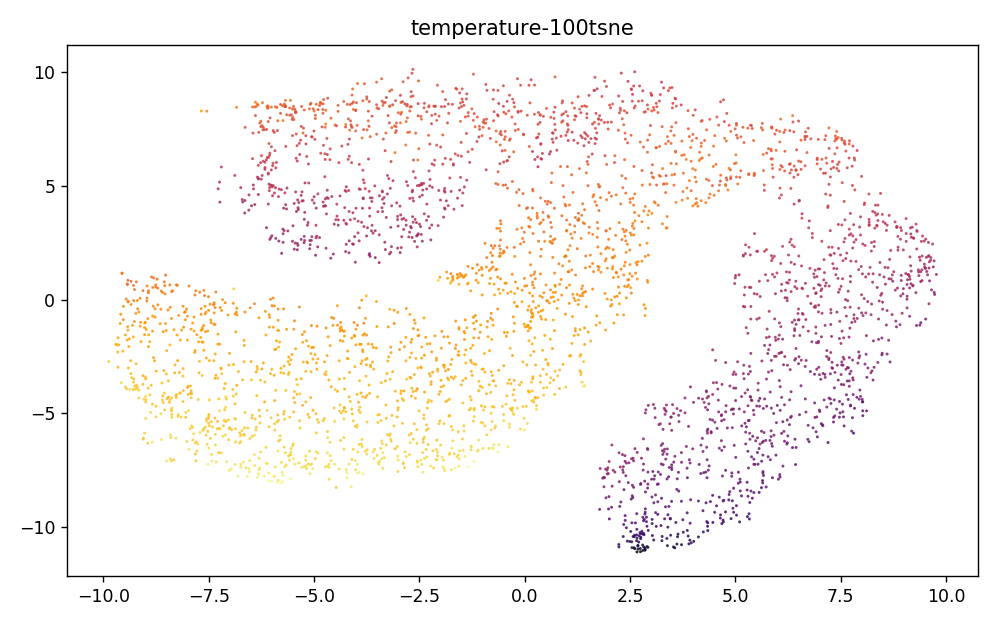
\includegraphics[width=\linewidth]{../png/vis/temperature-100tsne.png}
  \caption{tSNE on cleaned data from MDW, with p=100, colored by temp, using inferno colormap.}
  \label{fig:15tsne_temp}
\end{figure}


\section{Data Gathering and Cleaning}

I pulled all the data I used from the Weather Underground (wunderground.com) using one of their API's HTTP access points. I wrote a script and was able to retrieve daily weather data for four airports (SFO, MDW, LGA, ORD), from 1948 onwards. 

Not all of this data was immediately usable --- sometimes, data values for precipitation or other metrics were far beyond normal ranges, suggesting either freak storms, faulty readings, or simply human error in entering data. A few columns of the data were routinely null --- such as the "Events" column, that simply listed relevant qualitative labels for the day's weather ("Thunderstorm", "Foggy", etc.) Although potentially useful for later interpreting clusters, these data values were too sparse to be of much use for data collecting and analysis, and in addition, only represented information already present in the data itself (i.e. rainfall, humidity, windspeed, cloud cover). 

In addition, it quickly became clear that wind direction was too "strong" of a dimension, easily overridding variance from other dimensions. The fact that it was represented by an integer of degrees from 0 to 360 also meant that wind degrees near 0 and near 360, while actually simliar, are projected as far from another with any dimensionality reduction method. 

To solve this, I simply re-cast periodic information such as date and wind direction as vectors whose angle represents the current time of year or direction of wind. In addition, I scaled the wind vector by the wind speed, since lower wind speeds should reflect changes in wind direction. I left the date vector as-is, since I didn't use it in actual modelling, only for plotting purposes.
 
\begin{figure}[t]
  \centering
  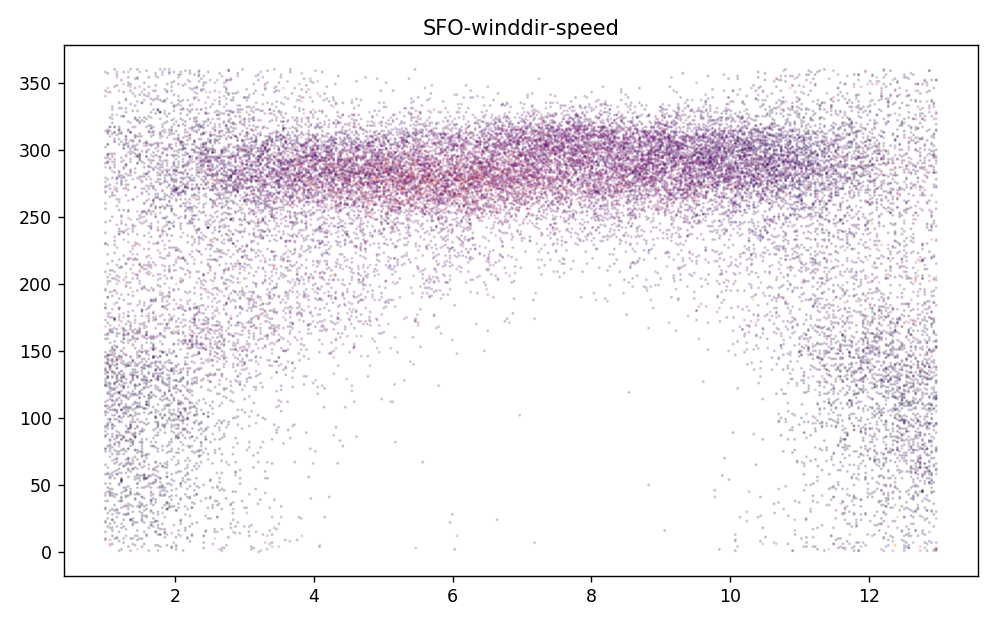
\includegraphics[width=\linewidth]{../png/basic-vis/SFO-winddir-speed.png}
  \caption{SFO wind dir by month --- color is speed}
  \label{fig:SFO_dir_speed}
\end{figure}


\begin{figure}[t]
  \centering
  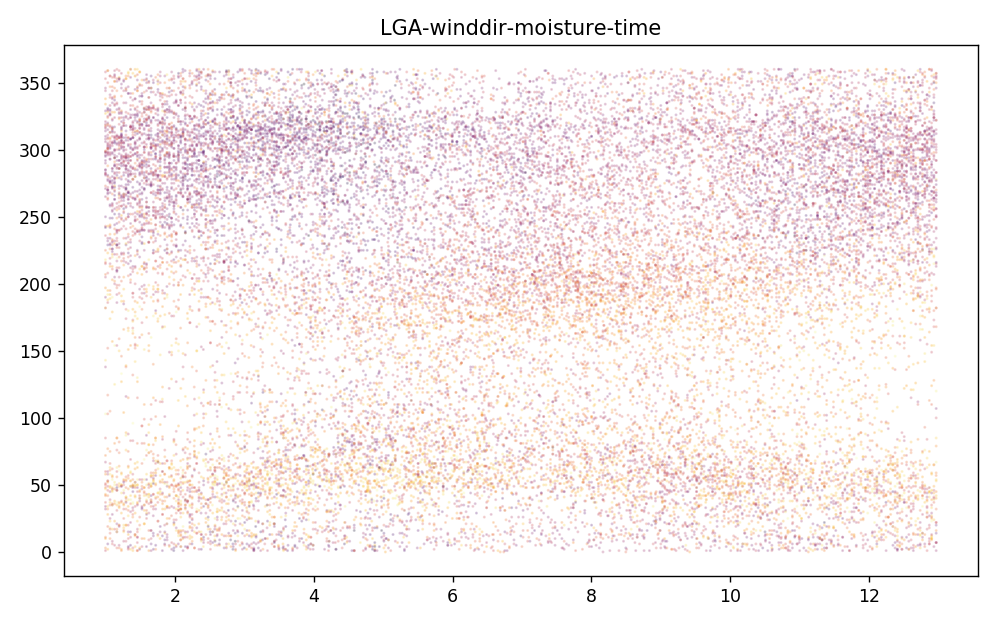
\includegraphics[width=\linewidth]{../png/basic-vis/LGA-winddir-moisture-time.png}
  \caption{LGA wind dir by month --- color is moisture}
  \label{fig:LGA_dir_moisture}
\end{figure}

\section{Data Visualizations}

It should first be noted that I'm using the \texttt{matplotlib}'s \texttt{\textbf{inferno}} colormap, which plots from dark purple through reddish, orange, and light yellow.

Given 20 dimensions of data, there isn't an immediately obvious "correct" axis to graph. Thus, I start off by applying both 2D and 3D PCA to the data, in addition to graphing a few interesting dimensions (I picked temperature, humidity, and windspeed) against time of year.

\subsection{Raw Data}
All of the simple graphs of the raw data showed similar, if not identical patterns; all cities seem to experience a minor month-long dip in humidity starting in April and October. Temperature peaks around August and is lowest in February. 

Perhaps the most interesting is wind direction (measured as the direction the wind is coming from, degrees clockwise from north) --- after re-converting the wind direction from vectors back to degrees, it appears that cities have different prevalent wind directions depending on the time of year. Of the airports I looked at, SFO (Figure~\ref{fig:SFO_dir_speed}) showed the greatest, clearest differences in wind direction; there's a specific cluster of weak winds for its "winter" (SF doesn't really have much of a winter, as is known), while the rest of the year has a very particular wind direction, with a standard deviation of about 20 degrees or so. Winds also typically seem strongest in the center of the cluster, though there are definitely many outliers. 

In addition, most of the points out-of-cluster seem to be of high humidity. LGA (Figure~\ref{fig:LGA_dir_moisture}) also showcases an effect where entire clusters have more humidity than other clusters; this is likely because, as LGA is on the coast, different wind directions can carry different amounts of moisture. This is likely the case for LGA, since the "dry" wind direction corresponds to northwest, the direction of the continental US, while the middle cluster (190 deg) points southwest along New Jersey, and the bottom year-round cluster (50 deg) points northeast along Connecticut. 


\subsection{Dimensionality Reduction, Clustering}

Running PCA on the data didn't exactly give much insight, besides how weather data has a lot of symmetric variation in a few metrics, and then lots of uneven distributions in other metrics. PCA in 3 dimensions simply returned a rough squashed ball, with the three dimensions representing wind direction, temperature, and humidity. 

On the other hand, tSNE gave some slightly better results. It was difficult to strike a balance between a large perplexity to reduce overclustering, and a small perplexity to pick out details --- since weather patterns aren't likely to be evenly distributed, too large of a perplexity would have ignored smaller weather patterns. In the end, I decided to err on the side of large perplexity. The smaller values kept giving me overclustered data roughly in the same shape as the large-perplexity tSNE. The result is Figure~\ref{fig:15tsne_temp}, of MDW. As you can see, the data is roughly continuous with temperature, as you'd expect --- temperature changes shouldn't happen too quickly. The data seems to roughly represent summer, winter, and an intermediary circular blob on top representing mid-fall and mid-spring (which are similar data-wise as you will see). 


\begin{figure}[t]
  \centering
  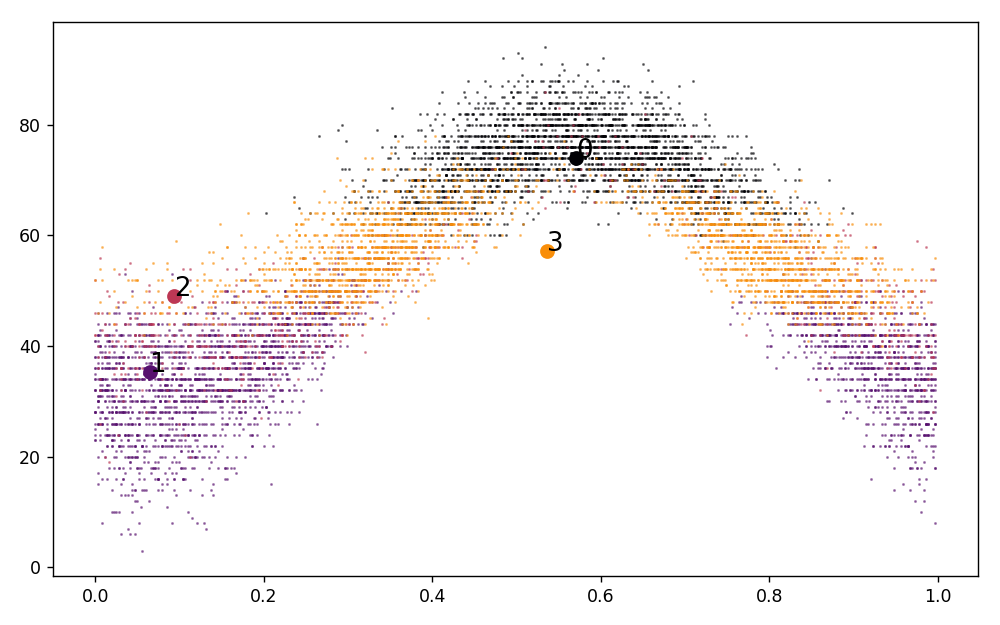
\includegraphics[width=\linewidth]{../png/models/LGA-basic-temperature4.png}
  \caption{LGA basic model, temp vs time}
  \label{fig:LGA_basics}
\end{figure}

\begin{table}[th]
  \caption{basic model state excerpt (LGA)}
  \label{tab:basic}
  \centering
  \begin{tabular}{c c c c c c}
    \toprule 
    \multicolumn{6}{c}{State means}\\
    State & MeanT & MeanH & MinV & Rain & Cloud \\
    \midrule
    $0$ & $74.1$   &  $67.93$  &  $4.78$  &  $0.0$    &   $2.54$ \\
    $1$ & $35.44$  &  $56.26$  &  $7.76$  &  $0.0$    &   $2.27$ \\
    $2$ & $48.95$  &  $87.13$  &  $1.73$  &  $0.46$   &   $4.57$ \\
    $3$ & $57.04$  &  $61.03$  &  $7.29$  &  $0.0$    &   $2.37$ \\
    \bottomrule
  \end{tabular}

  \begin{tabular}{c c c c c}
    \toprule
    \multicolumn{5}{c}{Transition matrix}\\
    Start & End 0 & End 1 & End 2 & End 3 \\
    \midrule  
    $0$ & $0.86$  &  $0.0 $  &  $0.03$  &  $0.11$ \\
    $1$ & $0.0 $  &  $0.83$  &  $0.08$  &  $0.09$ \\
    $2$ & $0.11$  &  $0.34$  &  $0.3 $  &  $0.24$ \\
    $3$ & $0.12$  &  $0.09$  &  $0.08$  &  $0.71$ \\
    \bottomrule
  \end{tabular}
\end{table} 




\section{HMM models, Analysis}

By far the most interesting analyses are to be found within analyzing the HMM models produced. I ran each model for each airport 5 times, for each number of hidden states $n=[2,4,6,8,10]$. For each model, in addition to examining the transition matrix and hidden state means, I also extracted the most likely sequence of states from the data, and graphed the state associated with each point (via color) on top of the actual point's location on the graph to aid in visualization. Some of these classes are easier to understand (like concat's classes) while others are a bit more obscure (like delta's classes), but each of them has its own reasoning hidden in the data. I decided to pull from LGA for all of these graphs simply because these illustrate my points the best --- all the other images are in the zip folder, within \texttt{png/models/}.


\subsection{Basic}

In this model, I simply trained the HMM model on the cleaned data.

As I increased the number of hidden states in the HMM, classes first started distinguishing themselvesvby temperature --- cold and warm. Beyond n=4, these states started to clearly distinguish themselves by humidity as well. As you can see in Figure~\ref{fig:LGA_basics}, three of the four states occupy very distinct sections of temperature (states 0, 1, and 3), while state 2 seems to hover above state 1, with points sparsely spread across the colder seasons.

By examining the states in the HMM (Figure~\ref{fig:LGA_basics}), we see that state 2 represents a storm on a cold, non-wintry day. It's the only state having a significant average rainfall, double the cloud coverage as the other states, and by far the greatest humidity and least visibility. By observing the transformation matrix, we also see that it is the only state that does not strongly refer back to itself, which makes sense --- the other three states can roughly represent seasons (or, in the case of state 3, two seasons), while state 2 represents what we can take to be a cold-front storm.

This state ended up doing the second-worst in the test (and not by a large margin either), right after the concatenated model. These two models both failed because the states ended up modelling the seasons more than the weather --- states 0, 1, and 3 in this model all refer strongly back to themselves, and the transition matrix ends up encoding more for season length than weather characteristics.





\subsection{Concatenated}
\begin{figure}[t]
  \centering
  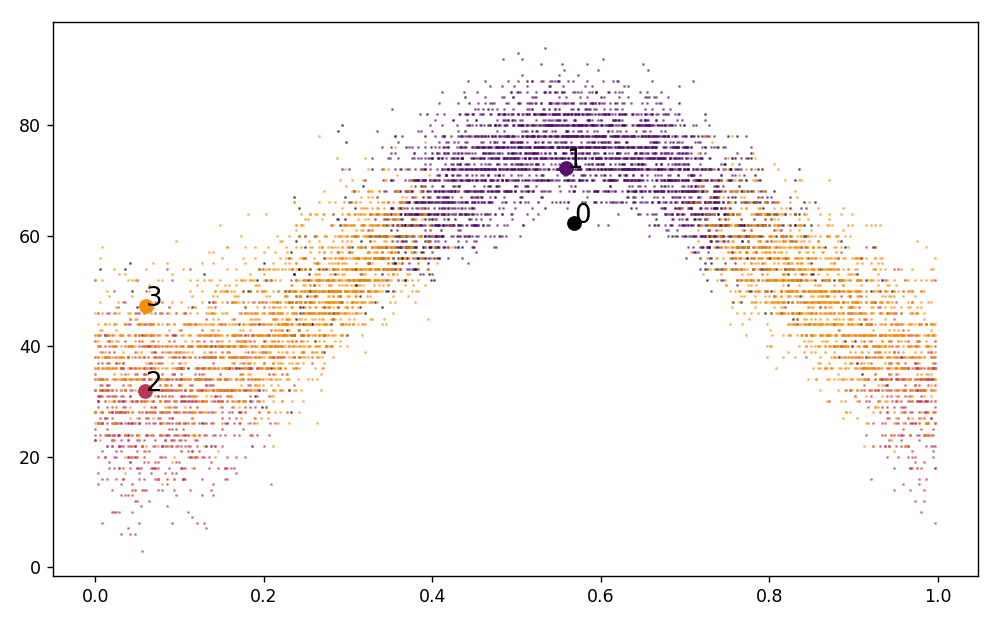
\includegraphics[width=\linewidth]{../png/models/LGA-concat-temperature4.png}
  \caption{LGA concat model, temp vs time}
  \label{fig:LGA_concat}
\end{figure}

In this model, I concatenated a week's worth of weather data together for each point --- thus, instead of a 21-dimension vector representing July 8, 1990, I had a 142-dimension vector representing July 8, 1990 that also had the past 6 days of weather data as well as July 8th's data. 

Looking at the results, this model was very similar to the basic model, except that everything was a little bit more separated on the time-axis. The concatenation of several weather states helped the model distinguish between different seasons as a result of multiple variables changing together (largely temperature and wind). Figure~\ref{fig:LGA_concat} displays this clearly --- the only difference between it and Figure~\ref{fig:LGA_basic} is that the class separations are vertical instead of horizontal --- time-separated instead of temperature-separated. However, this difference didn't seem to help the model learn a more abstract representation of the weather. In fact, it did slightly worse than basic on the benchmarks.

\subsection{Time-Independent}
\begin{figure}[t]
  \centering
  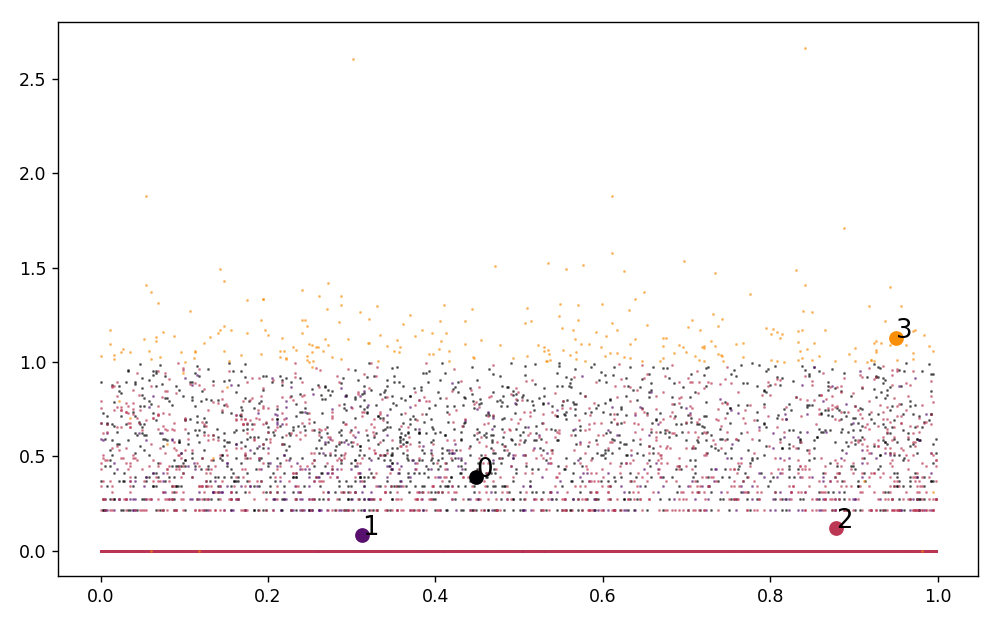
\includegraphics[width=\linewidth]{../png/models/LGA-timeless-cuberootrain4.png}
  \caption{LGA timeless model, cube root rainfall vs time}
  \label{fig:LGA_timeless_rain}
\end{figure}

For the time-independent model, I simply removed the temperature, dewpoint, and wind direction measurements in the data. Temperature and wind-direction are strongly correlated with time and year, and dewpoint is mostly just a combination of humidity and temperature anyways. 

Although this model didn't beat the naive model, it still ended up doing slightly better than the first two models. I believe the reason for that is in its states. Instead of being divided clearly along temperature or humidity, these states are very clearly divided into different levels of rain, and atmospheric pressures. The clear-cut divisions of atmospheric pressure is significant, because lower pressures strongly correspond to storms, while higher pressures strongly correspond to clear weather. 

As you can see in Figure~\ref{fig:LGA_timeless_rain}, state 3 represents all the days with rain beyond a constant threshold, and state 2 represents all the days without rain. Figure~\ref{fig:LGA_timeless_pressure} indicates the extremely clear-cut separation of atmospheric pressures between classes --- unsurprisingly, state 2 represents the days with high atmospheric pressure.


\begin{figure}[t]
  \centering
  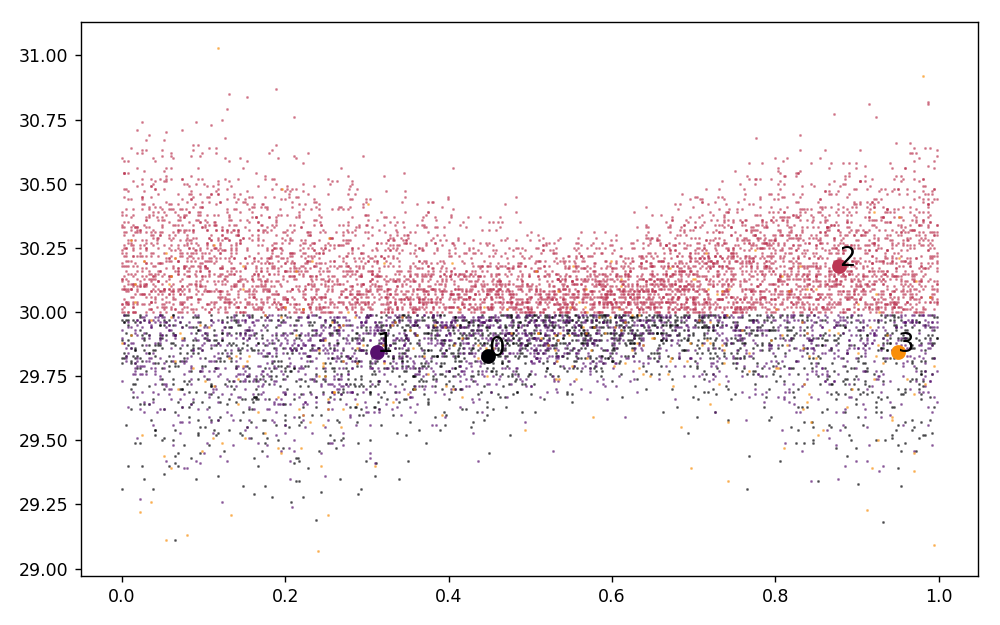
\includegraphics[width=\linewidth]{../png/models/LGA-timeless-pressure4.png}
  \caption{LGA timeless model, pressure vs time}
  \label{fig:LGA_timeless_pressure}
\end{figure}



\begin{table}[th]
  \caption{delta model state excerpt (LGA)}
  \label{tab:delta}
  \centering

  \begin{tabular}{c c c c c c c}
    \toprule 
    \multicolumn{7}{c}{State means}\\
      State&MeanT & MeanH & MeanV & MeanW & Rain & Cloud  \\
    \midrule
      0 & $ 0.46$  & $ 1.14 $ &  $-0.35$ &  $-0.29$  & $0.0$   &$ 0.1  $ \\
      1 & $-5.09$  & $-12.76$ &  $3.93 $ &  $3.26 $  & $-0.0$  &$-1.13 $  \\
    \bottomrule
  \end{tabular}

  \begin{tabular}{c c c}
    \toprule
    \multicolumn{3}{c}{Transition matrix}\\
    Start & End 0 & End 1 \\
    \midrule  
    0 & $0.93$ & $0.07$ \\
    1 & $0.73$ & $0.27$ \\
    \bottomrule
  \end{tabular}
\end{table}

\begin{figure}[t]
  \centering
  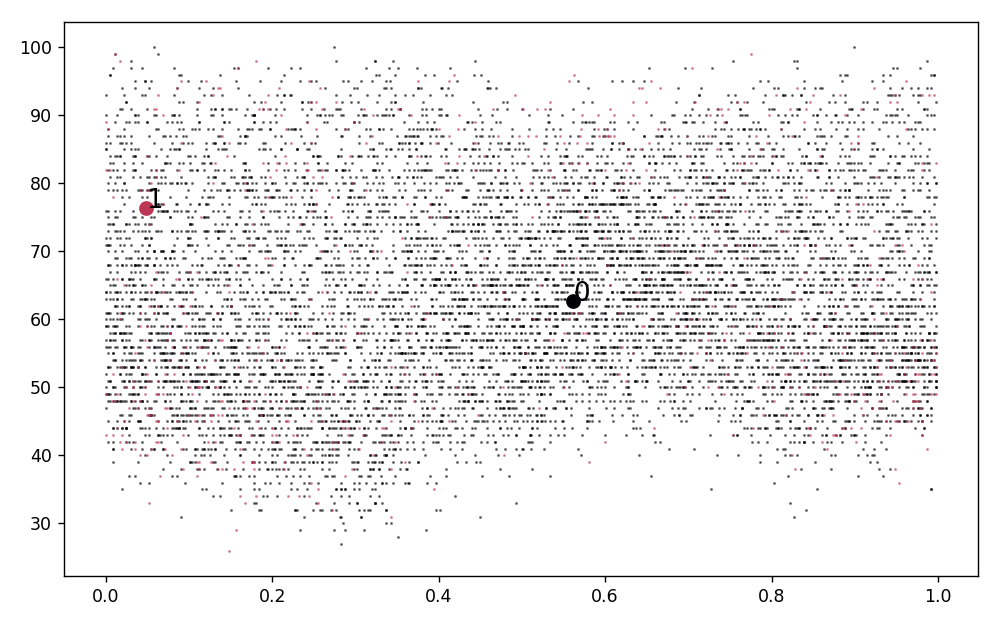
\includegraphics[width=\linewidth]{../png/models/LGA-delta-humidity2.png}
  \caption{LGA delta model, humidity vs time}
  \label{fig:LGA_delta}
\end{figure}

\begin{figure}[t]
  \centering
  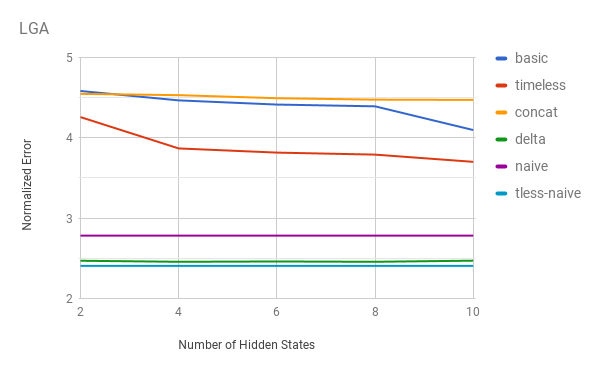
\includegraphics[width=\linewidth]{../png/analysis/LGA.png}
  \caption{LGA model errors}
  \label{fig:LGA_models}
\end{figure}



\subsection{Delta}


This model uses the deltas of the data instead of the data itself. That is, I compute the new input dataset as the old dataset minus the old dataset right-shifted by one, so that each entry in the new dataset represents the amount each dimension changed by since the day before it.

This is implicitly similar to the timeless model, since taking temperature and wind deltas significantly reduces their temporal dependency, but by taking deltas instead of removing information dimensions altogether, this method preserves more of the raw data.

If you look at Figure~\ref{fig:LGA_delta}, you'll see that these states don't seem to be easily discernable with respect to humidity. This actually makes sense --- since the model is trained off of humidity differences instead of absolute humidity, it is far more sensitive to humidity changes rather than total humidity. Humidity changes are also largely uncorrelated to total humidity, since humidity is a continuous variable under-the-hood. 

However, these two opaque states managed to beat the naive model by a small margin. In fact, for all airports, all delta models (for any number of hidden states I tested) beat the naive model. To understand why, we have to look at the model's transition matrix and state means in Table~\ref{tab:delta}.

State 0 refers to a slowly warming state, and state 1 refers to a rapid temperature drop. Since the temperature mostly stays consistent year to year (global warming is not yet rapid enough to affect that assumption), we know immediately that state 0 occurs about 10 times more than state 1. However, that also means that state 1 refers to a much more drastic change in state than state 0 --- humidity drops, visibility rises, rain decreases (although, negligbly), and clouds clear up.

These are all signs of a high-pressure system. Although other models have clearer states of "dry and cold" or "wet and rainy", with 2 states, the delta model has already uncovered high and low pressure systems. Now, note that these systems don't have to be absolute --- merely relative. The pressure vs time graph for the delta model doesn't outline a separation between high-pressure days and low-pressure days --- rather, the model learns pressure systems as a relative affect.



\section{Test Results and Conclusions}
As seen in Figure~\ref{fig:LGA_models} we have beat naive prediction. Professional national meteorology services routinely beat us, with average temperature differences of less than 1 degree F. However, local weather services routinely differ by up to 5 or 6 degrees F, and in that ballpark, our model is not so far off. 

Then again, neither is the naive model!
\\
\qquad
\\
\qquad
























\bibliographystyle{IEEEtran}

\bibliography{mybib}

\begin{thebibliography}{9}
\bibitem[1]{Davis80-COP}
  Audrey\ W.\ Zhu and Halton\ Pi
  ``A Method for Improving the Accuracy of Weather Forecasts Based on a Comprehensive Statistical Analysis of Historical Data for the Contiguous United States,''
  \textit{ J Climatol Weather Forecasting }, vol.~2, 2014.
\end{thebibliography}


\end{document}
